\section{Программная реализация задачи}

\href{https://github.com/utpwtb/ITMO/tree/main/4%20%D0%92%D1%8B%D1%87%D0%B8%D1%81%D0%BB%D0%B8%D1%82%D0%B5%D0%BB%D1%8C%D0%BD%D0%B0%D1%8F%20%D0%9C%D0%B0%D1%82%D0%B5%D0%BC%D0%B0%D1%82%D0%B8%D0%BA%D0%B0/%D0%9F%D1%80%D0%BE%D0%B3%D1%80%D0%B0%D0%BC%D0%BC%D0%B0/Lab4/CM_Lab4}{{\color{blue} GitHub - Лабораторная работа №4}}

\subsection{Архитектура программы}

Программа реализована на языке Java с графическим интерфейсом (Swing). Содержит следующие классы:

\begin{itemize}
\item \textbf{Main.java} — точка входа, запуск GUI.
\item \textbf{MainFrame.java} — главное окно с вкладками: ввод данных, результаты, графики.
\item \textbf{ChartPanel.java} — панель отрисовки графиков аппроксимирующих функций.
\item \textbf{LSMSolver.java} — ядро вычислений: метод наименьших квадратов для всех видов функций.
\item \textbf{ApproximationResult.java} — модель данных результата аппроксимации.
\item \textbf{BatchRunner.java} — пакетный режим для автоматической генерации графиков и отчётов.
\end{itemize}

\subsection{Метод наименьших квадратов (LSMSolver.java)}

\begin{lstlisting}[style=javaStyle, label=code:lsm]
public class LSMSolver {
    
    public static ApproximationResult linear(List<Double> x, List<Double> y) {
        int n = x.size();
        double sX = 0, sXX = 0, sY = 0, sXY = 0;
        for (int i = 0; i < n; i++) {
            double xi = x.get(i), yi = y.get(i);
            sX += xi; sXX += xi * xi; sY += yi; sXY += xi * yi;
        }
        double det = sXX * n - sX * sX;
        double a = (sXY * n - sX * sY) / det;
        double b = (sXX * sY - sX * sXY) / det;
        return buildResult("y = ax + b", x, y, xi -> a * xi + b, new double[]{a, b});
    }

    public static ApproximationResult quadratic(List<Double> x, List<Double> y) {
        // ... решение системы 3x3 методом Гаусса
    }

    public static ApproximationResult cubic(List<Double> x, List<Double> y) {
        // ... решение системы 4x4 методом Гаусса
    }

    public static ApproximationResult exponential(List<Double> x, List<Double> y) {
        // Линеаризация: ln(y) = ln(a) + bx
        List<Double> lnY = y.stream().map(Math::log).collect(Collectors.toList());
        ApproximationResult lin = linear(x, lnY);
        double a = Math.exp(lin.getCoefficients()[1]); // b -> ln(a)
        double b = lin.getCoefficients()[0];            // a -> b
        // ...
    }

    public static ApproximationResult logarithmic(List<Double> x, List<Double> y) {
        // Линеаризация: y = a*ln(x) + b
        List<Double> lnX = x.stream().map(Math::log).collect(Collectors.toList());
        ApproximationResult lin = linear(lnX, y);
        // ...
    }

    public static ApproximationResult power(List<Double> x, List<Double> y) {
        // Линеаризация: ln(y) = ln(a) + b*ln(x)
        List<Double> lnX = x.stream().map(Math::log).collect(Collectors.toList());
        List<Double> lnY = y.stream().map(Math::log).collect(Collectors.toList());
        ApproximationResult lin = linear(lnX, lnY);
        double a = Math.exp(lin.getCoefficients()[1]);
        double b = lin.getCoefficients()[0];
        // ...
    }
}
\end{lstlisting}

\subsection{Вычисление коэффициента детерминации $R^2$}

\[
R^2 = 1 - \frac{\sum_{i=1}^{n} (y_i - \varphi_i)^2}{\sum_{i=1}^{n} (y_i - \bar{y})^2},
\quad \bar{y} = \frac{1}{n}\sum_{i=1}^{n} y_i
\]

Программа выводит сообщение в зависимости от значения $R^2$:

\begin{itemize}
\item $R^2 \geq 0{,}95$ — «Высокая точность аппроксимации»
\item $0{,}75 \leq R^2 < 0{,}95$ — «Удовлетворительная аппроксимация»
\item $0{,}5 \leq R^2 < 0{,}75$ — «Слабая аппроксимация»
\item $R^2 < 0{,}5$ — «Точность аппроксимации недостаточна»
\end{itemize}

\subsection{Коэффициент корреляции Пирсона (для линейной аппроксимации)}

\[
r = \frac{\sum_{i=1}^{n} (x_i - \bar{x})(y_i - \bar{y})}
{\sqrt{\sum_{i=1}^{n} (x_i - \bar{x})^2 \cdot \sum_{i=1}^{n} (y_i - \bar{y})^2}}
\]

\subsection{Блок-схема алгоритма}

\begin{figure}[h]
    \centering
    \includegraphics[width=0.8\linewidth]{pic/Lab4.drawio.png}
    \caption{Блок-схема работы программы}
    \label{fig:flow}
\end{figure}

\newpage

\section{Пример работы программы}

\subsection{Тест 1 — Данные варианта 14}

Исходные данные: $y = \dfrac{25x}{x^4 + 14}$, $x \in [0, 4]$, $h=0{,}4$ (11 точек).

Результаты аппроксимации представлены в таблице~\ref{tab:test1} и на рисунке~\ref{fig:test1}.

\begin{figure}[h]
    \centering
    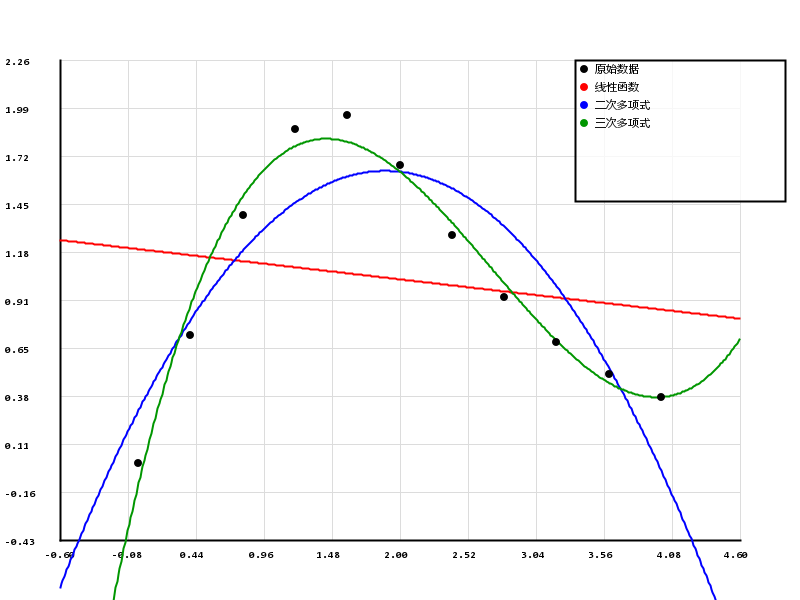
\includegraphics[width=0.9\linewidth]{pic/test1_chart.png}
    \caption{Графики аппроксимирующих функций (данные варианта 14)}
    \label{fig:test1}
\end{figure}

Для данного набора данных наилучшей аппроксимирующей функцией является кубическая ($\delta=0{,}095$), так как исходная функция не является полиномом невысокой степени. Экспоненциальная, логарифмическая и степенная функции не применимы из-за наличия точки $x=0$, $y=0$.

\subsection{Тест 2 — Данные лекционного примера}

Тестирование на данных лекции №4 (пример 3, 7 точек). Результаты совпадают с лекционными — коэффициенты аппроксимирующих функций идентичны.

\begin{figure}[h]
    \centering
    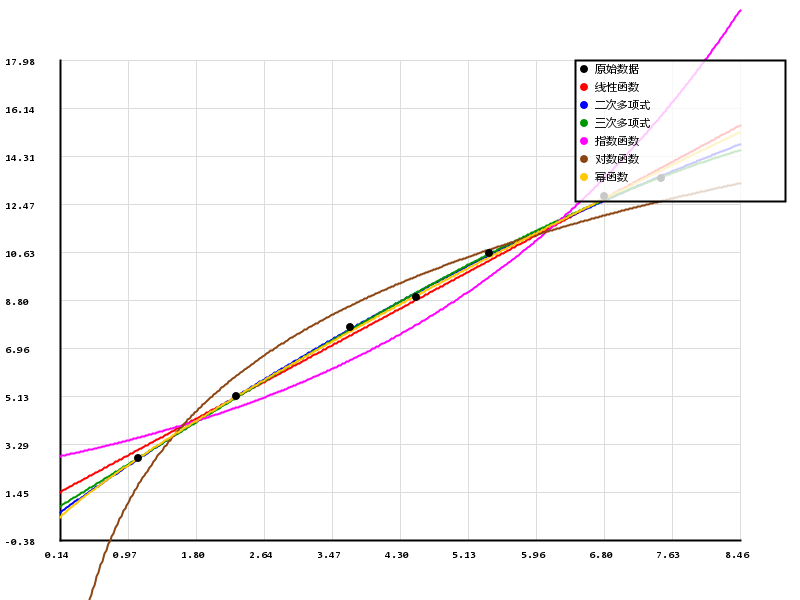
\includegraphics[width=0.9\linewidth]{pic/test2_chart.png}
    \caption{Графики аппроксимирующих функций (лекционный пример)}
    \label{fig:test2}
\end{figure}

\subsection{Тест 3 — Случайный набор данных}

Тест на линейно-подобных данных (10 точек с малым шумом). Линейная аппроксимация показывает $R^2=0{,}999$, что подтверждает высокую линейную зависимость.

\begin{figure}[h]
    \centering}
    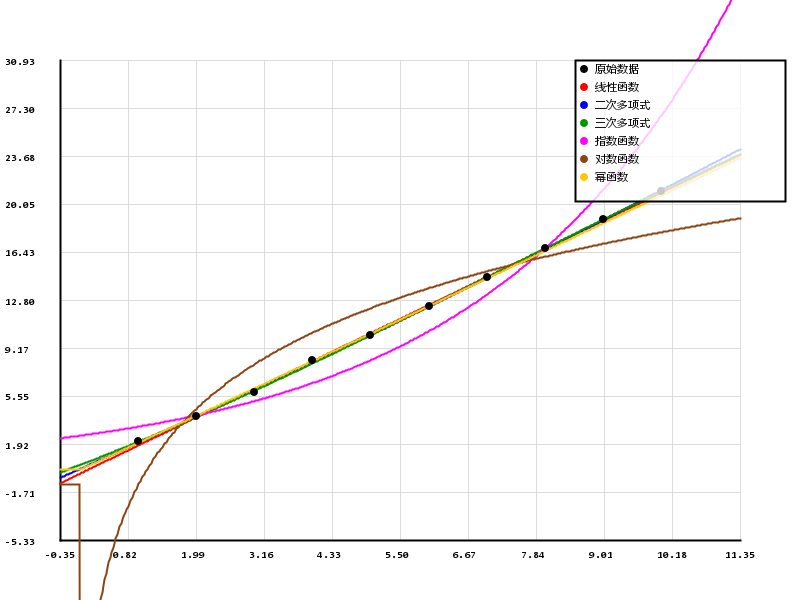
\includegraphics[width=0.9\linewidth]{pic/test3_chart.png}
    \caption{Графики аппроксимирующих функций (случайные данные)}
    \label{fig:test3}
\end{figure}

\section{Вывод}

В ходе выполнения лабораторной работы была изучена аппроксимация функций методом наименьших квадратов (МНК). В вычислительной части были построены линейная и квадратичная аппроксимации для заданной функции $y = 25x/(x^4+14)$ на интервале $[0, 4]$, найдены среднеквадратичные отклонения: $\delta_{\text{лин}} = 0{,}605$, $\delta_{\text{кв}} = 0{,}289$. Наилучшим из двух приближений является квадратичное.

В программной части реализовано приложение на Java с графическим интерфейсом (Swing), поддерживающее шесть видов аппроксимирующих функций: линейную, квадратичную, кубическую, экспоненциальную, логарифмическую и степенную. Программа вычисляет коэффициенты МНК, меру отклонения $S$, среднеквадратичное отклонение $\delta$, коэффициент корреляции Пирсона (для линейной аппроксимации) и коэффициент детерминации $R^2$ с выводом соответствующей оценки. Результаты отображаются в табличном виде и на графиках. Программа протестирована на различных наборах данных: данные варианта 14, данные лекционного примера и случайные данные, — и показала корректные результаты, согласующиеся с ручными вычислениями.
